\documentclass[12pt]{article}

\usepackage[]{amsmath}
\usepackage[]{amsthm}
\usepackage[]{amsfonts}
\usepackage[]{amssymb}
\usepackage{blindtext}
\usepackage[a4paper, total={7.5in, 10in}]{geometry}
\usepackage{graphicx}
\usepackage{listings}
\usepackage{color}
\usepackage{array}
\usepackage{wrapfig}
\usepackage{hyperref}

\definecolor{dkgreen}{rgb}{0,0.6,0}
\definecolor{gray}{rgb}{0.5,0.5,0.5}
\definecolor{mauve}{rgb}{0.58,0,0.82}

\pagenumbering{arabic}
\let\cleardoublepage\clearpage


%% parameters for code snippets, etc (to put a keywords and smaller snippets inline, use \texttt{} tag
\lstset{frame=tb,
  language=Java,
  aboveskip=3mm,
  belowskip=3mm,
  showstringspaces=false,
  columns=flexible,
  basicstyle={\small\ttfamily},
  numbers=left,
  numberstyle=\small\color{black},
  keywordstyle=\color{blue},
  commentstyle=\color{dkgreen},
  stringstyle=\color{mauve},
  breaklines=true,
  breakatwhitespace=true,
  tabsize=4
}

%%title of document
\title{Conceptual architecture analysis of OpenPilot}



%%ADD NAME AND STUDENT NUMBER HERE
\author{
    \textbf{Jerry Wu} (jerrywu0@my.yorku.ca), \textbf{Joseph Spagnuolo} (joe13@my.yorku.ca),\\ \textbf{Tarun Bhardwaj} (tarunb4@my.yorku.ca),
    \textbf{Krishna Raju} (krishnar@my.yorku.ca),\\ \textbf{Irsa Nasir} (inasi022@my.yorku.ca),
    \textbf{Aish Singh} (aish19@my.yorku.ca),\\ \textbf{Stanley Ihesiulo} (ihesiulo@my.yorku.ca),\\
    \textbf{Connor Francis McGrath} (connorm3@my.yorku.ca),
}



%%due date
\date{Due Feb 14 2024}



\begin{document}
\maketitle
\tableofcontents


\newpage


\section{Abstract}
This paper will outline the overarching architecture of the open source system "OpenPilot" by comma.ai.

\section{Introduction and Overview}

\subsection{The big picture}
Designed by comma.ai with the intent of increasing road safety, openpilot is an Advanced Driver Assistance System. It offers many driving safety features such as: Adaptive Cruise Control, Automatic Lane Centering, the ability to observe the attentiveness of the driver, and pathfinding capabilities that allow for automated steering and braking for other vehicles on the road [3].

The purpose of this report is to provide an analysis of the conceptual architecture of the openpilot. As will be discussed later, openpilot is the amalgamation of many different architecture systems, who in turn are composed of many different subsystems that take raw data from peripherals and hardware attached to the car, process the data, sends their output to a neural network which outputs commands that the car can execute [5]. This report will go into detail about the larger systems, their subsystems, the architectural styles that can be derived from their interactions with each other.

In order for the car to actually be controlled, openpilot takes advantage of the automobile’s CAN bus. The panda device allows the software to send the information collected from the peripherals to the mechanisms of the car [1]. This report will also describe the processes which convert the inputs from peripherals into actionable commands that can physically affect the vehicle.

Important to mention that this report will not just describe the software within the system, but the external interfaces the system retrieves information from, and the interfaces it outputs information to, such as the panda interface mentioned above, as well as devices such as the comma 3, which communicates with the panda interface [4], and is the hardware device that is physically mounted to the car, which the driver interacts with.

In order to demonstrate the capabilities of the openpilot system in the real world, this report will describe several concrete use cases of openpilot in action. The first describes how openpilot determines if it is safe to engage the system, describing how the software components are able to detect the condition of the driver and whether or not the system is safe enough to be engaged. The second use case demonstrates how the software components are able to provide tangible instructions to the CAN bus. This includes longitudinal information, that controls brakes and acceleration, and lateral information that controls steering.

However, it is not important to merely mention the current state of the system, but how comma.ai has set up a system that facilitates the evolution of future iterations of the openpilot system, through logging sensor data and compressed video to train and improve the neural network [5], as well as the open source github repository that welcomes contribution from all users [3].

In order to make the report more readable, naming conventions of the architecture, as well as key terms will be described.

To conclude, the report will also document the lessons learned from the group, as well as proposals for features that openpilot could incorporate into future iterations, or improvements to the existing systems, as well as what the group could have done differently in our exploration of the openpilot software system.
\newpage
\begin{figure}[ht]
    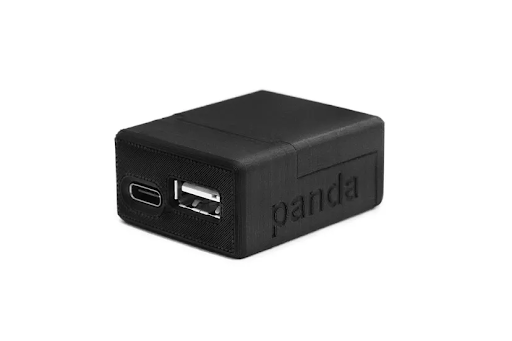
\includegraphics[scale=0.5]{Assets/panda.png}\\
    \caption{The most pretty panda yet. 9 Oct. 2019. Comma-Ai.medium.com, Medium,\\ \url{https://comma-ai.medium.com/our-hardware-future-eea980d8c3bd. Accessed 9 Feb. 2024.}}
    \label{fig:enter-label}
\end{figure}
This is the panda interface system that allows openpilot to send the information collected from the peripherals to be transferred to the car. It also allows the comma device to connect to the vehicle [1].




\subsection{Components and architecture}

Give the overall structure of the studied system, with descriptions of each major component and the interactions among them. These components are to be primarily subsystems or modules, but may also include threads or processes, files, and databases. In your descriptions, concentrate on goals, requirements, evolvability, testability, etc., rather than on lower-level concepts such as classes, variables and control flow. Discuss any parts of the system that are performance critical, i.e., which might not run fast enough. Discuss how the architecture supports future changes in the system. You should clarify global control flow, such as units of concurrency and method of passing control from one component to another. Your system's architecture should be easy to understand, with simple interfaces, and modest interactions among subsystems and modules. Clarify the architectural style (in the sense of Garlan and Shaw) that characterizes the overall system and its various parts. You are not to concentrate on minor components, such as classes and procedures, which are smaller than packages or modules. However, you may wish to discuss important abstractions, patterns, classes, data structures or algorithms that are critical to the success of the architecture.


\begin{itemize}

    \item \textbf{Architectures used}
    \begin{itemize}
        \item The software utilizes an implicit invocation architecture which can be found in their use of cereal; comma.ai's own open source library for robotic message communication. %Implicit invocation architecture (found in their use of cereal; an open source library for robotic message communication)
        \item Implicit invocation is also used in the boardd class which acts as the "publisher". The class manages messages sent/received to/from the panda module.
         \item A pipe and filter architecture is exhibited when data from sensors and actuators in the car itself are fed through openpilot's logic and processed by the neural networks working behind the scenes. %Pipe & filter (data is fed into the system via the sensors and processed by neural networks) 
        \item This may be unrelated, but the open source codebase is stored on a GitHub repository, so this could also be a repository style architecture for when developers are working on the project.
    \end{itemize}

    \item \textbf{Components}
    \begin{itemize}
        \item Sensors + actuators (boardd, camerad, sensord, etc.)
        \item Neural network runners (modeId, dmonitoringmodeId, dmonitoringd, etc.)
        \item Localization + calibration (locationd, calibrationd, etc.)
        \item Controls (radard, planners, controlsd, etc.
        \item System logging/misc (manager, thermald, etc.)
        \item Hardware components (panda module)
    \end{itemize}
\end{itemize}

\subsection{Architecture in depth}

\begin{itemize}
    \item \textbf{General OpenPilot Architecture}: 
    \\In general, OpenPilot can be depicted as a layered style architecture which contains 8 layers.
    \begin{itemize}
        \item Layer 1: Vehicle Interface 
        \item Layer 2: Communication and Data Interpretation
        \item Layer 3: Sensing and Actuation
        \item Layer 4: Core Neural Network Runners
        \item Layer 5: Localization and Calibration \item Layer 6: Control Algorithms
        \item Layer 7: System Management and Logging
        \item Layer 8: User Interface and Experience 
    \end{itemize} 
    \begin{figure}[ht]
        \centering
        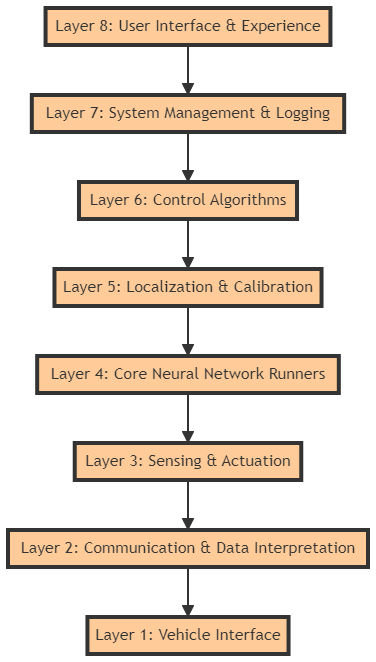
\includegraphics[scale=0.5]{Assets/layers.png}\\
        \caption{A bottom up diagram detailing the general architecture of openpilot}
        \label{fig:enter-label}
    \end{figure}

    \begin{itemize}
        \item The \textbf{vehicle interface layer} includes the car’s hardware and peripherals that interface with OpenPilot. This includes \textbf{CAN} (Controller Area Network) interface which enables communication with the car’s internal network, \textbf{steering wheel angle} sensor measures angle of steering wheel, \textbf{camera} provides visual input around the vehicle, \textbf{IMU} (Inertial Measurement Unit) also provides movement and orientation information, \textbf{GNSS Receiver} provides global positioning data, and along with other vehicle sensors that are used to ensure the vehicle is functioning properly.
    
        \item The \textbf{communication and data interpretation layer} consists of libraries like opendbc which interprets CAN bus data based on \textbf{DBC} files, \textbf{panda} which is hardware that is used to read/write from and to the CAN bus, \textbf{laika} which processes \textbf{GPS} data for more precise positioning, and \textbf{cereal} which is the message protocol for inter-process communication.
        
        \item The \textbf{sensing and actuation layer} includes \textbf{boardd} which manages communication between the panda and the openpilot software, \textbf{camerad} which processes image data from the car’s cameras, and \textbf{sensord} which handles IMU and additional sensor data reading. All together this layer manages the direct interaction with the car’s hardware and the data from the sensors.
        
        \item The \textbf{core neural network runners layer} includes \textbf{modeld} which runs the driving policy in order for the neural network to make driving decisions, \textbf{dmonitoringmodeld} which runs the driver monitoring neural network to ensure that the driver is paying attention, \textbf{dmonitoringd} which contains logic to see whether the driver can take over the wheel if necessary. Overall, this layer runs the neural networks which are responsible for driving and driver monitoring.
        
        \item The \textbf{localization and calibration layer} includes \textbf{ubloxd} which parses GNSS data for localization, \textbf{locationd} which uses a Kalman filter service to provide precise vehicle localization, \textbf{calibrationd} which calibrates the camera to align it with the vehicle’s frame, and \textbf{paramsd} which adjusts the vehicle parameters for more accurate control.
        
        \item The \textbf{control algorithms layer} uses \textbf{radard} which processes radar data for detecting objects and tracking them, \textbf{plannerd} which laterally and longitudinally calculates the path planning, and \textbf{controlsd} which generates and sends the control commands to the actuators of the vehicle.

        \item The \textbf{system management and logging layer} contains \textbf{manager} which oversees the lifecycle of openpilot services, \textbf{thermald} which monitors the thermal state of the device and ensures it does not overheat, \textbf{loggerd} which records driving and analyses that data for improvements, \textbf{logcatd} which logs system messages and errors, \textbf{proclogd} which logs detailed process data, and \textbf{athenad} which manages the connection to common.ai services for updates and any remote assistance.
        
        \item Lastly, \textbf{the user interface and experience layer} has a \textbf{UI} which is in charge of displaying the interface for the user, including a live camera feed, system alerts and status.  
    \end{itemize}

    \item \textbf{Global control flow} %%FINISH THIS
    
    \item \textbf{Concurrency}
    \begin{itemize}
        \item \textbf{Concurrent testing}: Utilises the \textbf{pytest} module to achieve parallelization and streamline test suite execution. This allows for concurrent testing, maximising resource use and minimising idle time. 
        \item \textbf{Driving controls system}: The control system handled by the \textbf{controlsd} module is responsible for managing autonomous vehicle operations, it relies on concurrent data from other modules and is responsible for executing crucial driving functions including acceleration, braking, and steering.
        \item \textbf{Driver monitoring system}: The driver monitoring system handled by the \textbf{dmonitoringd} is responsible to ensure the driver remains alert, It ensures driver attentiveness and readiness to take control when necessary. It concurrently processes data provided by a machine learning model, and video data to decide if the driver needs to be alerted.

    \end{itemize}

\end{itemize}


\subsection{How do these components interact?}

\section{Diagrams}

\begin{figure}[ht]
    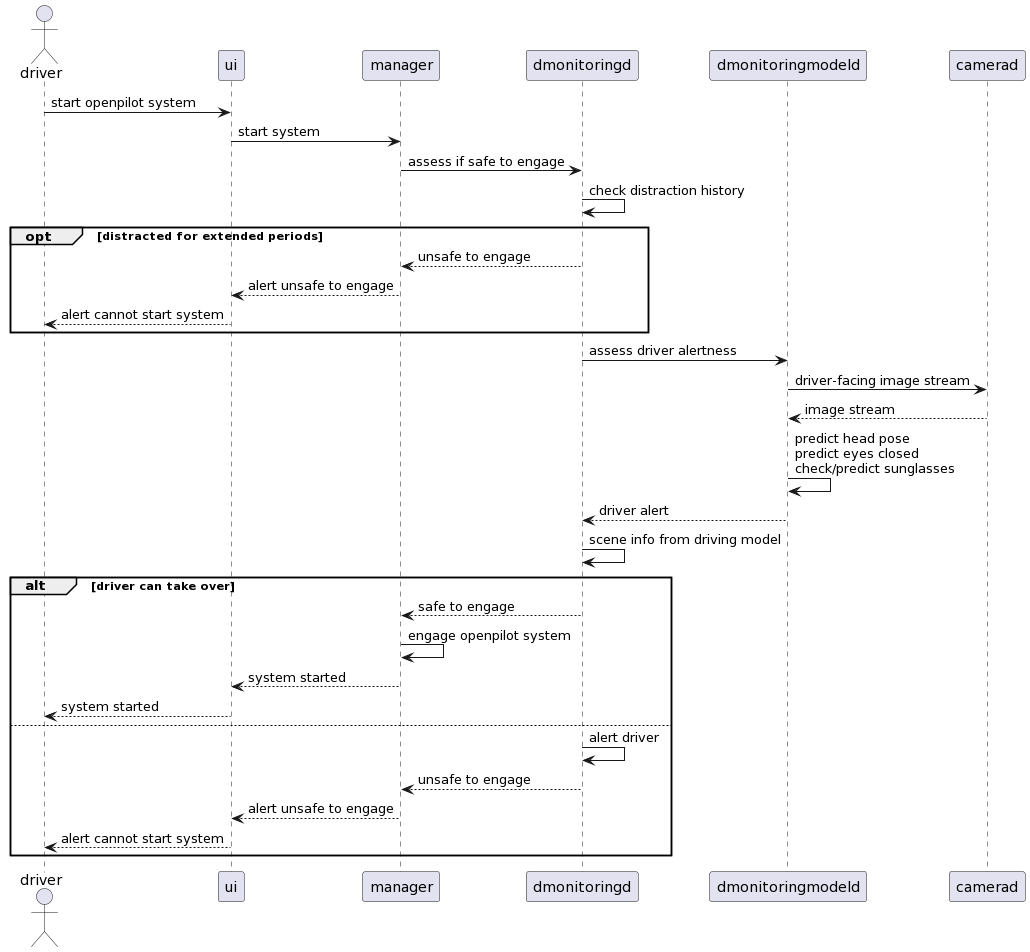
\includegraphics[scale=0.4]{Assets/sequence.png}
    \\
    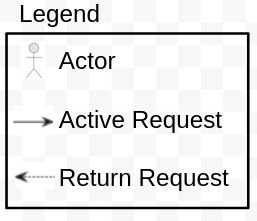
\includegraphics[scale=0.4]{Assets/legend.png}
    \caption{A sequence diagram detailing a case where a driver becomes distracted while openpilot is active}
    \label{fig:enter-label}
\end{figure}

\section{External Interfaces}

\section{Use Cases}

\section{Data Dictionary}

\section{Naming Conventions}

\section{Conclusion}

\section{Lessons learned and Alternatives Presented}

\begin{thebibliography}{00}

    \bibitem{b1} S. Anumakonda, “The state of comma.ai,” Medium.com, \url{https://srianumakonda.medium.com/the-state-of-comma-ai-2140aabc6f52} (accessed Feb. 13, 2024).

    \bibitem{b2} “openpilot 0.9.5,” comma.ai, \url{https://blog.comma.ai/095release/} (accessed Feb. 13, 2024).

    \bibitem{b3} “Openpilot - Open source advanced driver assistance system,” comma.ai, \url{https://comma.ai/openpilot} (accessed Feb. 13, 2024).

    \bibitem{b4} “From vision to architecture: How to use openpilot and live,” From Vision To Architecture: How to use openpilot and live - DESOSA 2020, \url{https://desosa.nl/projects/openpilot/2020/03/11/from-vision-to-architecture} (accessed Feb. 13, 2024).

    \bibitem{b5} “How openpilot works in 2021,” comma.ai, \url{https://blog.comma.ai/openpilot-in-2021/} (accessed Feb. 13, 2024). 

    \bibitem{b6} “Comma 3x - make driving chill,” comma.ai, \url{https://comma.ai/shop/comma-3x} (accessed Feb. 13, 2024). 
\end{thebibliography}

\end{document}